% Copyright 2018 by Till Tantau
%
% This file may be distributed and/or modified
%
% 1. under the LaTeX Project Public License and/or
% 2. under the GNU Free Documentation License.
%
% See the file doc/generic/pgf/licenses/LICENSE for more details.


\section{Guidelines on Graphics\\关于图形的指导原则}

The present section is not about \pgfname\ or \tikzname, but about general
guidelines and principles concerning the creation of graphics for scientific
presentations, papers, and books.

本节内容不涉及\pgfname\ 或 \tikzname,而是关于为科学演示、论文和书籍创建图形的一般指导原则。

The guidelines in this section come from different sources. Many of them are
just what I would like to claim is ``common sense'', some reflect my personal
experience (though, hopefully, not my personal preferences), some come from
books (the bibliography is still missing, sorry) on graphic design and
typography. The most influential source  are the brilliant books by Edward
Tufte. While I do not agree with everything written in these books, many of
Tufte's arguments are so convincing that I decided to repeat them in the
following guidelines.

本节中的指导原则来自不同的来源。其中许多只是我想称之为“常识”的东西,一些反映了我的个人经验(虽然希望不是我的个人偏好),一些来自于关于平面设计和排版的书籍(参考文献尚缺,抱歉)。最有影响力的来源是Edward Tufte的出色著作。虽然我不同意这些书中的所有观点,但Tufte的许多论点非常有说服力,因此我决定在下面的指导原则中重复它们。

The first thing you should ask yourself when someone presents a bunch of
guidelines is: Should I really follow these guidelines? This is an important
question, because there are good reasons not to follow general guidelines. The
person who set up the guidelines may have had other objectives than you do. For
example, a guideline might say ``use the color red for emphasis''. While this
guideline makes perfect sense for, say, a presentation using a projector, red
``color'' has the \emph{opposite} effect of ``emphasis'' when printed using a
black-and-white printer. Guidelines were almost always set up to address a
specific situation. If you are not in this situation, following a guideline can
do more harm than good.

当有人提出一系列指导原则时,你应该问自己一个重要的问题:我真的需要遵循这些指导原则吗?这是一个重要的问题,因为有很多理由不遵循通用指导原则。设定指导原则的人可能有与你不同的目标。例如,一个指导原则可能说“使用红色强调”。虽然这个指导原则对于使用投影仪的演示非常合理,但使用黑白打印机打印时,红色“颜色”与“强调”的效果恰恰相反。指导原则几乎总是为了应对特定情况而设定的。如果你不处于这种情况下,遵循指导原则可能会弊大于利。

The second thing you should be aware of is the basic rule of typography is:
``Every rule can be broken, as long as you are \emph{aware} that you are
breaking a rule.'' This rule also applies to graphics. Phrased differently, the
basic rule states: ``The only mistakes in typography are things done in
ignorance.'' When you are aware of a rule and when you decide that breaking the
rule has a desirable effect, break the rule.

第二件你应该知道的事情是排版的基本规则是:“只要你知道你正在违反规则,每条规则都可以被打破。”这条规则也适用于图形。换句话说,基本规则是:“在无知的情况下,印刷错误。”当你了解一条规则并决定违反规则会产生期望的效果时,你就可以打破这条规则。


\subsection{Planning the Time Needed for the Creation of Graphics\\计划创建图形所需的时间}

When you create a paper with numerous graphics, the time needed to create these
graphics becomes an important factor. How much time should you calculate for
the creation of graphics?

当你创建一篇包含多个图形的论文时,创建这些图形所需的时间成为一个重要因素。你应该为创建图形计算多少时间?

As a general rule, assume that a graphic will need as much time to create as
would a text of the same length. For example, when I write a paper, I need
about one hour per page for the first draft. Later, I need between two and four
hours per page for revisions. Thus, I expect to need about half an hour for the
creation of \emph{a first draft} of a half page graphic. Later on, I expect
another one to two hours before the final graphic is finished.

一般原则是,假设创建一个图形所需的时间与创建同样长度的文本所需的时间相同。例如,当我写一篇论文时,我需要为初稿每页用时约一小时。之后,我每页的修订时间为两到四个小时。因此,我预计为创建半页图形的\emph{初稿}需要大约半小时。之后,我预计还需要一到两个小时才能完成最终的图形。

In many publications, even in good journals, the authors and editors have
obviously  invested a lot of time on the text, but seem to have spend about
five minutes to create all of the graphics. Graphics often seem to have been
added as an ``afterthought'' or look like a screen shot of whatever the
authors's statistical software shows them. As will be argued later on, the
graphics that programs like \textsc{gnuplot} produce by default are of poor
quality.

在许多出版物中,即使是在好的期刊中,作者和编辑明显在文本上投入了很多时间,但在创建所有图形上似乎只花了约五分钟的时间。图形通常看起来像是“事后想法”,或者像是作者统计软件的屏幕截图。正如后面将要论述的那样,像\textsc{gnuplot}这样的程序默认生成的图形质量较差。

Creating informative graphics that help the reader and that fit together with
the main text is a difficult, lengthy process.

创建有助于读者并与主要文本配合的信息图形是一个困难而耗时的过程。
%
\begin{itemize}
    \item Treat graphics as first-class citizens of your papers. They deserve
        as much time and energy as the text does. Indeed, the creation of
        graphics might deserve \emph{even more} time than the writing of the
        main text since more attention will be paid to the graphics and they
        will be looked at first.

        将图形视为论文中的重要组成部分。它们应该得到与文本一样的时间和精力对待。实际上,创建图形可能需要比撰写主要文本更多的时间,因为图形会受到更多的关注,读者会首先看到它们。

    \item Plan as much time for the creation and revision of a graphic as you
        would plan for text of the same size.

        为创建和修订一个图形安排与相同大小的文本所需的时间相同。


    \item Difficult graphics with a high information density may require even
        more time.

        信息密度较高的复杂图形可能需要更多时间。


    \item Very simple graphics will require less time, but most likely you do
        not want to have ``very simple graphics'' in your paper, anyway; just
        as you would not like to have a ``very simple text'' of the same
        size.

        非常简单的图形所需的时间较少,但是在论文中你可能不希望有“非常简单的图形”,就像你不希望有与其大小相同的“非常简单的文本”一样。


\end{itemize}


\subsection{Workflow for Creating a Graphic\\创建图形的工作流程}

When you write a (scientific) paper, you will most likely follow the following
pattern: You have some results/ideas that you would like to report about. The
creation of the paper will typically start with compiling a rough outline.
Then, the different sections are filled with text to create a first draft. This
draft is then revised repeatedly until, often after substantial revision, a
final paper results. In a good journal paper there is typically not be a single
sentence that has survived unmodified from the first draft.

当你撰写一篇(科学)论文时,你很可能会按照以下模式进行:你有一些结果/想法需要报告。创建论文通常从编写一个大致的大纲开始。然后,不同的部分填充文本以创建初稿。然后,这个草稿将反复修订,通常经过大幅修改,最终形成最终的论文。在一篇好的期刊论文中,通常没有一个句子是完全未经修改的。

Creating a graphics follows the same pattern:

创建图形遵循相同的模式:
%
\begin{itemize}
    \item Decide on what the graphic should communicate. Make this a
        conscious decision, that is, determine ``What is the graphic supposed
        to tell the reader?''

        确定图形应该传达的内容。这是一个有意识的决定,即确定“图形应该告诉读者什么?”


    \item Create an ``outline'', that is, the rough overall ``shape'' of the
        graphic, containing the most crucial elements. Often, it is useful to
        do this using pencil and paper.

        创建“大纲”,即粗略的图形“形状”,包含最关键的元素。通常,使用铅笔和纸张进行此操作是有用的。


    \item Fill out the finer details of the graphic to create a first draft.

    填写图形的细节,创建初稿。


    \item Revise the graphic repeatedly along with the rest of the paper.

    与论文的其余部分一起反复修订图形。
\end{itemize}


\subsection{Linking Graphics With the Main Text\\将图形与主要文本联系起来}

Graphics can be placed at different places in a text. Either, they can be
inlined, meaning they are somewhere ``in the middle of the text'' or they can
be placed in stand-alone ``figures''. Since printers (the people) like to have
their pages ``filled'', (both for aesthetic and economic reasons) stand-alone
figures may traditionally be placed on pages in the document far away from the
main text that refers to them. \LaTeX\ and \TeX\ tend to encourage this
``drifting away'' of graphics for technical reasons.

图形可以放置在文本的不同位置。它们可以嵌入,即它们在“文本中间的某个位置”,或者它们可以放在独立的“图形”中。由于印刷机(人)喜欢将页面“填满”(无论是出于美观还是经济原因),独立的图形传统上可能会被放置在离引用它们的主文本很远的文档页面上。出于技术原因,\LaTeX\ 和 \TeX\ 倾向于鼓励图形“漂移”。

When a graphic is inlined, it will more or less automatically be linked with
the main text in the sense that the labels of the graphic will be implicitly
explained by the surrounding text. Also, the main text will typically make it
clear what the graphic is about and what is shown.

当图形嵌入时,它们将自动与主文本相关联,因为图形的标签将通过周围的文本隐式解释。此外,主文本通常会清楚地说明图形的内容和显示内容。

Quite differently, a stand-alone figure will often be viewed at a time when the
main text that this graphic belongs to either has not yet been read or has been
read some time ago. For this reason, you should follow the following guidelines
when creating stand-alone figures:

相比之下,独立的图形通常在主文本还没有被阅读或已经被阅读一段时间后才被查看。因此,在创建独立图形时,应遵循以下准则:
%
\begin{itemize}
    \item Stand-alone figures should have a caption than should make them
        ``understandable by themselves''.

        独立图形应该有一个标题,使它们“自解释”。

        For example, suppose a graphic shows an example of the different
        stages of a quicksort algorithm. Then the figure's caption should, at
        the very least, inform the reader that ``the figure shows the
        different stages of the quicksort algorithm introduced on page xyz''.
        and not just ``Quicksort algorithm''.

        例如,假设一个图形显示快速排序算法的不同阶段的示例。那么图形的标题应该至少告诉读者“该图示了在第xyz页介绍的快速排序算法的不同阶段”。而不仅仅是“快速排序算法”。
    \item A good caption adds as much context information as possible. For
        example, you could say: ``The figure shows the different stages of
        the quicksort algorithm introduced on page xyz. In the first line,
        the pivot element 5 is chosen. This causes\dots'' While this
        information can also be given in the main text, putting it in the
        caption will ensure that the context is kept. Do not feel afraid of a
        5-line caption. (Your editor may hate you for this. Consider hating
        them back.)

        一个好的标题应该尽可能添加上下文信息。例如,你可以说:“该图示了在第xyz页介绍的快速排序算法的不同阶段。第一行中选择了枢轴元素5。这导致……”虽然这些信息也可以在主文本中提供,但将其放在标题中将确保保留上下文。不要害怕一个有5行标题。(你的编辑可能会讨厌你这样做。考虑讨厌他们。)
    \item Reference the graphic in your main text as in ``for an example of
        quicksort `in action', see Figure~2.1 on page xyz''.

        在主文本中引用图形,例如:“有关快速排序的示例,请参见第2.1图,第xyz页。”


    \item Most books on style and typography recommend that you do not use
        abbreviations as in ``Fig.~2.1'' but write ``Figure~2.1''.

        大多数关于样式和排版的书籍建议不要使用缩写,例如“Fig.~2.1”,而应写成“图~2.1”。


        The main argument against abbreviations is that ``a period is too
        valuable to waste it on an abbreviation''. The idea is that a period
        will make the reader assume that the sentence ends after ``Fig'' and
        it takes a ``conscious backtracking'' to realize that the sentence
        did not end after all.

        缩写的主要反对理由是“用句号浪费太多宝贵的空间”。观点是句号会让读者认为句子在“Fig”后结束,需要进行“有意识的倒退”才能意识到句子并没有结束。


        The argument in favor of abbreviations is that they save space.

        支持缩写的论据是它们可以节省空间。


        Personally, I am not really convinced by either argument. On the one
        hand, I have not yet seen any hard evidence that abbreviations slow
        readers down. On the other hand, abbreviating all ``Figure'' by
        ``Fig.'' is most unlikely to save even a single line in most documents.
        I avoid abbreviations.

        就个人而言,我并不完全相信这两种论点。一方面,我尚未看到任何确凿的证据表明缩写会减慢读者的阅读速度。另一方面,大多数文档中缩写所有“Figure”的方式不太可能节省一行,因此我避免使用缩写。

\end{itemize}


\subsection{Consistency Between Graphics and Text\\图形与文本之间的一致性}

Perhaps the most common ``mistake'' people do when creating graphics (remember
that a ``mistake'' in design is always just ``ignorance'') is to have a
mismatch between the way their graphics look and the way their text looks.

创建图形时,人们经常犯的最常见的“错误”(记住在设计中,“错误”始终只是“无知”)是图形的外观与文本的外观不匹配。


It is quite common that authors use several different programs for creating the
graphics of a paper. An author might produce some plots using \textsc{gnuplot},
a diagram using \textsc{xfig}, and include an |.eps| graphic a coauthor
contributed using some unknown program. All these graphics will, most likely,
use different line widths, different fonts, and have different sizes. In
addition, authors often use options like |[height=5cm]| when including graphics
to scale them to some ``nice size''.

通常情况下,作者使用多个不同的程序创建论文的图形。一个作者可能使用\textsc{gnuplot}创建一些图,使用\textsc{xfig}创建一个图表,并包含一个由合著者使用某个未知程序贡献的|.eps|图形。所有这些图形很可能使用不同的线宽、不同的字体和不同的大小。此外,作者在包含图形时经常使用|[height=5cm]|等选项将其缩放到某个“合适的大小”。

If the same approach were taken to writing the main text, every section would
be written in a different font at a different size. In some sections all
theorems would be underlined, in another they would be printed all in uppercase
letters, and in another in red. In addition, the margins would be different on
each page. Readers and editors would not tolerate a text if it were written in
this fashion, but with graphics they often have to.

如果以相同的方式撰写主文本,每个部分都将使用不同的字体以不同的大小编写。在某些部分,所有定理都会被划线,在另一些部分,它们将全部以大写字母打印,在另一些部分则以红色打印。此外,每页的边距也会有所不同。读者和编辑不会接受这种方式编写的文本,但是对于图形,他们经常不得不接受。

To create consistency between graphics and text, stick to the following
guidelines:

为了在图形和文本之间创建一致性,请遵循以下准则:
%
\begin{itemize}
    \item Do not scale graphics.

    不要缩放图形。



        This means that when generating graphics using an external program,
        create them ``at the right size''.

        这意味着在使用外部程序生成图形时,要以“正确的大小”创建它们。

    \item Use the same font(s) both in graphics and the body text.

    在文本和图形中使用相同的字体。


    \item Use the same line width in text and graphics.

    在文本和图形中使用相同的线宽。


        The ``line width'' for normal text is the width of the stem of letters
        like T{}. For \TeX, this is usually $0.4\,\mathrm{pt}$. However, some
        journals will not accept graphics with a normal line width below
        $0.5\,\mathrm{pt}$.

        “正常文本的线宽”是字母的笔干的宽度,如 T{}。对于 \TeX,这通常是$0.4\,\mathrm{pt}$。然而,一些期刊不接受正常线宽小于$0.5\,\mathrm{pt}$的图形。

    \item When using colors, use a consistent color coding in the text and in
        graphics. For example, if red is supposed to alert the reader to
        something in the main text, use red also in graphics for important
        parts of the graphic. If blue is used for structural elements like
        headlines and section titles, use blue also for structural elements
        of your graphic.

        使用颜色时,在文本和图形中使用一致的颜色编码。例如,如果红色用于引起读者的注意,在图形中也使用红色来突出显示图形的重要部分。如果蓝色用于结构元素(如标题和章节标题),在图形的结构元素中也使用蓝色。


        However, graphics may also use a logical intrinsic color
        coding. For example, no matter what colors you normally use, readers
        will generally assume, say, that the color green as ``positive, go,
        ok'' and red as ``alert, warning, action''.

        然而,图形也可以使用逻辑的内在颜色编码。例如,无论你通常使用什么颜色,读者通常会认为绿色表示“积极、前进、正常”,红色表示“警告、危险、行动”。

\end{itemize}

Creating consistency when using different graphic programs is almost
impossible. For this reason, you should consider sticking to a single graphics
program.

当使用不同的图形程序时,几乎不可能实现一致性。因此,你应该考虑坚持使用单一的图形程序。

\subsection{Labels in Graphics\\图形中的标签}

Almost all graphics will contain labels, that is, pieces of text that explain
parts of the graphics. When placing labels, stick to the following guidelines:

几乎所有的图形都包含标签,即解释图形的部分的文本。在放置标签时,请遵循以下准则:
%
\begin{itemize}
    \item Follow the rule of consistency when placing labels. You should do
        so in two ways: First, be consistent with the main text, that is, use
        the same font as the main text also for labels. Second, be consistent
        between labels, that is, if you format some labels in some particular
        way, format all labels in this way.

        在遵循一致性规则放置标签时,你应该从两个方面考虑:首先,与主文本保持一致,即在标签中使用与主文本相同的字体。其次,标签之间要保持一致,即如果以某种特定方式格式化某些标签,那么所有标签都应以这种方式格式化。


    \item In addition to using the same fonts in text and graphics, you
        should also use the same notation. For example, if you write $1/2$ in
        your main text, also use ``$1/2$'' as labels in graphics, not
        ``0.5''. A $\pi$ is a ``$\pi$'' and not ``$3.141$''. Finally,
        $\mathrm e^{-\mathrm i \pi}$ is ``$\mathrm e^{-\mathrm i \pi}$'', not
        ``$-1$'', let alone ``-1''.

        除了在文本和图形中使用相同的字体之外,你还应该使用相同的符号。例如,如果在主文本中写$1/2$,则在图形中的标签中也使用“$1/2$”,而不是“0.5”。$\pi$是“$\pi$”,而不是“$3.141$”。最后,$\mathrm e^{-\mathrm i \pi}$是“$\mathrm e^{-\mathrm i \pi}$”,而不是“$-1$”,更不用说“-1”了。


    \item Labels should be legible. They should not only have a reasonably
        large size, they also should not be obscured by lines or other text.
        This also applies to labels of lines and text \emph{behind} the
        labels.

        标签应该是可读的。它们不仅应该具有合理的大小,而且还不应被线条或其他文本遮挡。这也适用于线条和文本“在标签后面”时的标签。


    \item Labels should be ``in  place''. Whenever there is enough space,
        labels should be placed next to the thing they label. Only if
        necessary, add a (subdued) line from the label to the labeled object.
        Try to avoid labels that only reference explanations in external
        legends. Reader have to jump back and forth between the explanation and
        the object that is described.

        标签应该“放在适当的位置”。只要有足够的空间,标签应该放在它们所标记的对象旁边。只有在必要的情况下,才添加一个(柔和的)线段将标签与被标记的对象连接起来。尽量避免仅引用外部图例中的解释的标签。读者必须在解释和描述对象之间来回跳转。


    \item Consider subduing ``unimportant'' labels using, for example, a gray
        color. This will keep the focus on the actual graphic.

        考虑用灰色颜色减弱“不重要”的标签。这将保持对实际图形的关注。


\end{itemize}


\subsection{Plots and Charts\\绘图和图表}

One of the most frequent kind of graphics, especially in scientific papers, are
\emph{plots}. They come in a large variety, including simple line plots,
parametric plots, three dimensional plots, pie charts, and many more.

科学论文中最常见的图形类型之一是\emph{绘图}。绘图有很多不同的类型,包括简单的折线图、参数图、三维图、饼图等等。


Unfortunately, plots are notoriously hard to get right. Partly, the default
settings of programs like \textsc{gnuplot} or Excel are to blame for this since
these programs make it very convenient to create bad plots.

不幸的是,绘图是非常难做到完美的。部分原因是像\textsc{gnuplot}或Excel这样的程序的默认设置,因为这些程序非常方便地创建糟糕的绘图。


The first question you should ask yourself when creating a plot is: Are there
enough data points to merit a plot? If the answer is ``not really'', use a
table.

在创建绘图时,你应该问自己的第一个问题是:是否有足够的数据点来证明是值得绘制图表的?如果答案是“实际上没有”,那就使用表格。

A typical situation where a plot is unnecessary is when people present a few
numbers in a bar diagram. Here is a real-life example: At the end of a seminar
a lecturer asked the participants for feedback. Of the 50 participants, 30
returned the feedback form. According to the feedback, three participants
considered the seminar ``very good'', nine considered it ``good'', ten ``ok'',
eight ``bad'', and no one thought that the seminar was ``very bad''.

一个典型的不需要绘图的情况是当人们在柱状图中呈现几个数字时。以下是一个真实例子:在研讨会结束时,演讲者要求参与者提供反馈。在50名参与者中,有30人回交反馈表。根据反馈,三位参与者认为研讨会“非常好”,九人认为研讨会“好”,十人认为研讨会“还行”,八人认为研讨会“差”,没有人认为研讨会“非常差”。

A simple way of summing up this information is the following table:

总结这些信息的一种简单方法是以下表格:

\medskip
\begin{tabular}{lp{3.75cm}r}
  \emph{Rating given} & \raggedright\emph{Participants (out of 50) who gave this rating} &
  \emph{Percentage} \\[1.75em]
  ``very good'' & \hfil\hphantom{0}3\hfil & \hphantom{0}6\% \\
  ``good'' & \hfil\hphantom{0}9\hfil & 18\% \\
  ``ok'' & \hfil10\hfil & 20\% \\
  ``bad'' & \hfil\hphantom{0}8\hfil & 16\% \\
  ``very bad'' & \hfil\hphantom{0}0\hfil & \hphantom{0}0\% \\[2mm]
  none & \hfil20\hfil & 40\% \\
\end{tabular}

\bigskip
What the lecturer did was to visualize the data using a 3D bar diagram. It
looked like this (except that in reality the numbers where typeset using some
extremely low-resolution bitmap font and were near-unreadable):

演讲者所做的是使用一个3D柱状图将数据进行可视化。它看起来像这样(实际上,数字使用一种极低分辨率的位图字体排版,并且几乎无法阅读):

\bigskip
\par
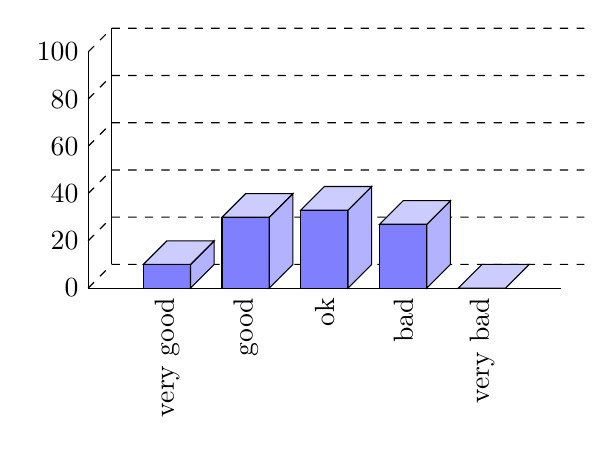
\begin{tikzpicture}[y=0.03cm,z=3mm]
  \foreach \y in {0,20,40,60,80,100}
    \draw[dashed] (0,\y,0) node[left] {\y} -- (0,\y,1)  -- (6,\y,1);

  \draw (0,0,0) -- (0,100,0)  (0,0,1) -- (0,100,1);
  \draw (0,0,0) -- (6,0,0);

  \foreach \x/\xtext/\height in {1/very good/10,2/good/30,3/ok/33,4/bad/27,5/very bad/0}
  {
    \draw (\x,0) node[rotate=90,anchor=east] {\xtext};

    \begin{scope}[xshift=\x cm]

    \filldraw[fill=blue!50] (-.3,0,0) rectangle (.3,\height,0);
    \filldraw[fill=blue!30] (.3,0,0) -- (.3,0,1) -- (.3,\height,1) -- (.3,\height,0) --cycle;
    \filldraw[fill=blue!20] (-.3,\height,0) -- (.3,\height,0) --
    (.3,\height,1) -- (-.3,\height,1) --cycle;
    \end{scope}
  }
\end{tikzpicture}
\bigskip

Both the table and the ``plot'' have about the same size. If your first thought
is ``the graphic looks nicer than the table'', try to answer the following
questions based on the information in the table or in the graphic:

表格和“图表”的大小几乎相同。如果你的第一个想法是“图形看起来比表格好看”,那么请回答以下问题,基于表格或图形中的信息:
%
\begin{enumerate}
    \item How many participants were there?

    有多少参与者?
    \item How many participants returned the feedback form?

    有多少参与者回交反馈表?
    \item What percentage of the participants returned the feedback form?

    回交反馈表的参与者占总参与者的百分比是多少?
    \item How many participants checked ``very good''?

    有多少参与者选择“非常好”?
    \item What percentage out of all participants checked ``very good''?

    在所有参与者中,选择“非常好”的百分比是多少?
    \item Did more than a quarter of the participants check ``bad'' or ``very
        bad''?

        有超过四分之一的参与者选择“差”或“非常差”吗?
    \item What percentage of the participants that returned the form checked
        ``very good''?

        返回表格的参与者中,选择“非常好”的百分比是多少?
\end{enumerate}

Sadly, the graphic does not allow us to answer \emph{a single one of these
questions}. The table answers all of them directly, except for the last one. In
essence, the information density of the graphic is very close to zero. The
table has a much higher information density; despite the fact that it uses
quite a lot of white space to present a few numbers. Here is the list of things
that went wrong with the 3D-bar diagram:


不幸的是,图形无法回答\emph{任何一个}这些问题。表格直接回答了所有这些问题,除了最后一个。从本质上讲,图形的信息密度接近零。表格的信息密度更高,尽管它使用大量的空白空间来呈现少量的数字。以下是3D柱状图出现问题的列表:
%
\begin{itemize}
    \item The whole graphic is dominated by irritating background lines.

    整个图形被令人讨厌的背景线所主导。
    \item It is not clear what the numbers at the left mean; presumably
        percentages, but it might also be the absolute number of
        participants.

    不清楚左侧的数字的含义;可能是百分比,但也可能是参与者的绝对人数。
    \item The labels at the bottom are rotated, making them hard to read.

    底部的标签是旋转的,很难阅读。



        (In the real presentation that I saw, the text was rendered at a very
        low resolution with about 10 by 6 pixels per letter with wrong
        kerning, making the rotated text almost impossible to read.)

        (在我看到的真实演示中,文本以非常低的分辨率呈现,每个字母约有10x6像素,并且字距错误,使旋转的文本几乎无法阅读。)


    \item The third dimension adds complexity to the graphic without adding
        information.

        第三个维度增加了图形的复杂性,但没有增加信息。


    \item The three dimensional setup makes it much harder to gauge the
        height of the bars correctly. Consider the ``bad'' bar. It the number
        this bar stands for more than 20 or less? While the front of the bar
        is below the 20 line, the back of the bar (which counts) is above.

        三维设置使得准确判断柱状图的高度变得更加困难。考虑一下这个“不好的”柱状图。这个柱状图代表的数字是大于20还是小于20?虽然柱状图的正面低于20线,但背面(计数的部分)却高于20线。




    \item It is impossible to tell which  numbers are represented by the
        bars. Thus, the bars needlessly hide the information these bars are
        all about.

        无法确定条形图代表的具体数字。因此,条形图无意中隐藏了这些条形图所代表的信息。


    \item What do the bar heights add up to? Is it 100\% or 60\%?

    条形的高度加起来是多少?是100\%还是60\%?


    \item Does the bar for ``very bad'' represent 0 or~1?

    “非常糟糕”这个条形图代表的是0还是1?


    \item Why are the bars blue?

    为什么条形是蓝色的?


\end{itemize}

You might argue that in the example the exact numbers are not important for the
graphic. The important things is the ``message'', which is that there are more
``very good'' and ``good'' ratings than ``bad'' and ``very bad''. However, to
convey this message either use a sentence that says so or use a graphic that
conveys this message more clearly:

你可能会辩称,在这个例子中,具体的数字对于图形来说并不重要。重要的是“信息”,即“非常好”和“好”的评分比“差”和“非常差”的评分多。然而,要传达这个信息,可以使用一句话来表达,或者使用一个更清晰地传达这个信息的图形:

\medskip
\par
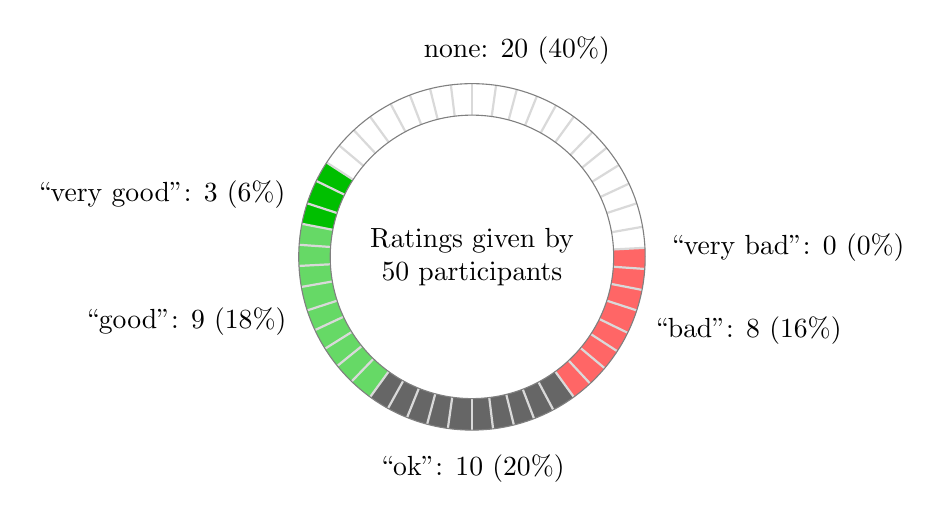
\begin{tikzpicture}
  \colorlet{good}{green!75!black}
  \colorlet{bad}{red}
  \colorlet{neutral}{black!60}
  \colorlet{none}{white}

  \node[align=center,text width=3cm]{Ratings given by 50~participants};

  \begin{scope}[line width=4mm,rotate=270]
    \draw[good]          (-123:2cm) arc (-123:-101:2cm);
    \draw[good!60!white] (-36:2cm) arc (-36:-101:2cm);
    \draw[neutral]       (-36:2cm) arc (-36:36:2cm);
    \draw[bad!60!white]  (36:2cm)  arc (36:93:2cm);

    \newcount\mycount
    \foreach \angle in {0,72,...,3599}
    {
      \mycount=\angle\relax
      \divide\mycount by 10\relax
      \draw[black!15,thick] (\the\mycount:18mm) -- (\the\mycount:22mm);
    }

    \draw (0:2.2cm) node[below] {``ok'': 10 (20\%)};
    \draw (165:2.2cm) node[above] {none: 20 (40\%)};
    \draw (-111:2.2cm) node[left] {``very good'': 3 (6\%)};
    \draw (-68:2.2cm) node[left] {``good'': 9 (18\%)};
    \draw (65:2.2cm) node[right] {``bad'': 8 (16\%)};
    \draw (93:2.2cm) node[right] {``very bad'': 0 (0\%)};
  \end{scope}
  \draw[gray] (0,0) circle (2.2cm) circle (1.8cm);
\end{tikzpicture}

\bigskip
The above graphic has about the same information density as the table (about
the same size and the same numbers are shown). In addition, one can directly
``see'' that there are more good or very good ratings than bad ones. One can
also ``see'' that the number of people who gave no rating at all is not
negligible, which is quite common for feedback forms.

上面的图形与表格具有大致相同的信息密度(大小相近,显示的数字相同)。此外,人们可以直接“看到”,“非常好”或“好”的评分比差评多。人们还可以“看到”,没有给出任何评分的人数并不可忽视,这在反馈表中很常见。

Charts are not always a good idea. Let us look at an example that I redrew from
a pie chart in \emph{Die Zeit}, June 4th, 2005:

图表并不总是一个好主意。让我们看一个我从《Die Zeit》2005年6月4日的饼图中重绘的例子:

\bigskip
\par
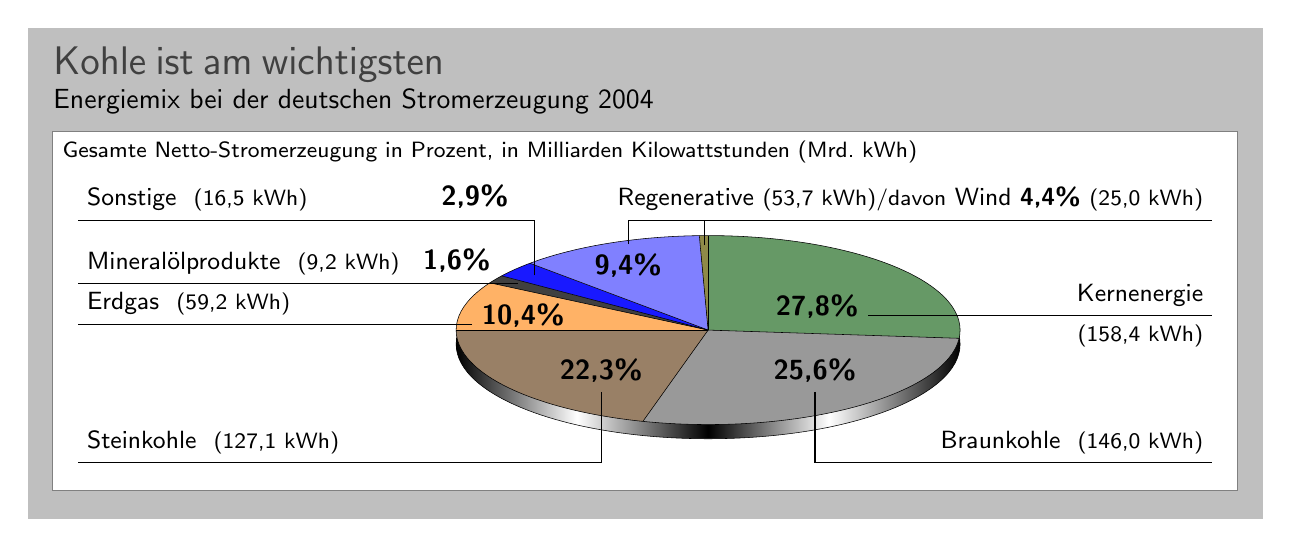
\begin{tikzpicture}
  \begin{scope}[xscale=3.2,yscale=1.2]

    \sffamily
    \coordinate (right border) at (2.0cm,-1.7cm);
    \coordinate (left border)  at (-2.5cm,2.1cm);

    \fill[black!25] ([xshift=-2mm,yshift=1.1cm]left border) rectangle ([xshift=2mm,yshift=-.3cm]right border);

    \node[below right,text width=10cm,inner sep=0pt] at ([yshift=.9cm,xshift=-1mm]left border)
    { {\color{black!75} \Large Kohle ist am wichtigsten}\\
      Energiemix bei der deutschen Stromerzeugung 2004};

    \filldraw[draw=gray,fill=white] ([xshift=-1mm]left border) node[below right,black]
      {\footnotesize Gesamte Netto-Stromerzeugung in Prozent, in
        Milliarden Kilowattstunden (Mrd.\ kWh)}
      rectangle ([xshift=1mm]right border);

    % The 3D stuff
    \pgfdeclarehorizontalshading{zeit}{100bp}
    {color(0pt)=(black);
      color(25bp)=(black);
      color(37bp)=(white);
      color(50bp)=(black);
      color(62bp)=(white);
      color(75bp)=(black);
      color(100bp)=(black)}

    \shadedraw[very thin,shading=zeit,yshift=-1.5mm] (0,0) circle (1cm);

    \fill[green!20!gray]   (0,0) -- (90:1cm) arc (90:-5:1cm);
    \fill[white!20!gray]   (0,0) -- (-5:1cm) arc (-5:-105:1cm);
    \fill[orange!20!gray]  (0,0) -- (-105:1cm) arc (-105:-180:1cm);
    \fill[orange!60!white] (0,0) -- (180:1cm) arc (180:150:1cm);
    \fill[black!75!white]  (0,0) -- (150:1cm) arc (150:145:1cm);
    \fill[blue!90!white]   (0,0) -- (145:1cm) arc (145:135:1cm);
    \fill[blue!50!white]   (0,0) -- (135:1cm) arc (135:92:1cm);
    \fill[yellow!50!black] (0,0) -- (92:1cm) arc (92:90:1cm);

    \begin{scope}[very thin]
      \draw (0,0) -- (90:1cm);
      \draw (0,0) -- (-5:1cm);
      \draw (0,0) -- (-105:1cm);
      \draw (0,0) -- (-180:1cm);
      \draw (0,0) -- (150:1cm);
      \draw (0,0) -- (145:1cm);
      \draw (0,0) -- (135:1cm);
      \draw (0,0) -- (92:1cm);

      \draw(0,0) circle (1cm);
    \end{scope}

    \node (Regenerative)   at (115:.75cm)  {\bfseries 9,4\%};
    \node (Kernenergie)    at (30:.5cm)   {\bfseries 27,8\%};
    \node (Braunkohle)     at (-45:.6cm)  {\bfseries 25,6\%};
    \node (Steinkohle)     at (-135:.6cm) {\bfseries 22,3\%};
    \node (Erdgas)         at (168:.75cm) {\bfseries 10,4\%};
    \coordinate (Mineral)  at (147:.9cm);
    \coordinate (Sonstige) at (140:.9cm);

    \small
    \draw (Regenerative.north) |- ([yshift=.25cm]Regenerative.north -| right border) coordinate (Regenerative label);
    \draw (91:.9cm) |- (Regenerative label);
    \node[above left] at (Regenerative label) {Regenerative\
      {\footnotesize (53,7 kWh)/davon} Wind \textbf{4,4\%}  \footnotesize (25,0 kWh)};

    \draw (Kernenergie.base east) -- (Kernenergie.base east -| right border) coordinate (Kernenergie label);
    \node[above left] at (Kernenergie label) {Kernenergie};
    \node[below left] at (Kernenergie label) {\footnotesize (158,4 kWh)};

    \draw (Braunkohle.south) |- ([yshift=-.75cm]Braunkohle.south -| right border) coordinate (Braunkohle label);
    \node[above left] at (Braunkohle label) {Braunkohle\ \ \footnotesize (146,0 kWh)};

    \draw (Steinkohle.south) |- ([yshift=-.75cm]Steinkohle.south -| left border) coordinate (Steinkohle label);
    \node[above right] at (Steinkohle label) {Steinkohle\ \ \footnotesize (127,1 kWh)};

    \draw (Erdgas.base west) -- (Erdgas.base west -| left border) coordinate (Erdgas label);
    \node[above right] at (Erdgas label) {Erdgas\ \ \footnotesize (59,2 kWh)};

    \draw (Mineral) -- (Mineral -| left border) coordinate (Mineral label);
    \node[above right] at (Mineral label) {Mineral\"olprodukte\ \
      \footnotesize (9,2 kWh) \  \ \normalsize\textbf{1,6\%}};

    \draw (Sonstige) |- (Regenerative label -| left border) coordinate (Sonstige label);
    \node[above right] at (Sonstige label) {Sonstige\ \
      \footnotesize (16,5 kWh) \hskip1.5cm\
      \normalsize\textbf{2,9\%}};
  \end{scope}
\end{tikzpicture}

This graphic has been redrawn in \tikzname, but the original looks almost
exactly the same.

这个图形是用\tikzname 重新绘制的,但原图看起来几乎完全相同。

At first sight, the graphic looks ``nice and informative'', but there are a lot
of things that went wrong:

乍一看,这个图形看起来“漂亮且信息丰富”,但有很多问题:

%
\begin{itemize}
    \item The chart is three dimensional. However, the shadings add nothing
        ``information-wise'', at best, they distract.

        图表是三维的。然而,阴影在“信息方面”没有任何作用,充其量只会分散注意力。

    \item In a 3D-pie-chart the relative sizes are very strongly distorted.
        For example, the area taken up by the gray color of ``Braunkohle'' is
        larger than the area taken up by the green color of ``Kernenergie''
        \emph{despite the fact that the percentage of Braunkohle is less than
        the percentage of Kernenergie}.

        在三维饼图中,相对大小被严重扭曲。例如,“褐煤”的灰色区域的面积大于“核能”的绿色区域的面积,尽管褐煤的百分比小于核能的百分比。


    \item The 3D-distortion gets worse for small areas. The area of
        ``Regenerative'' somewhat larger  than the area of ``Erdgas''. The
        area of ``Wind'' is slightly smaller than the area of
        ``Mineral\"olprodukte'' \emph{although the percentage of Wind is
        nearly three times larger than the percentage of
        Mineral\"olprodukte.}

        对于小面积,三维扭曲会更严重。与“天然气”相比,“再生能源”的面积稍大。尽管风能的百分比几乎是矿物油产品的三倍,但风能的面积略小于矿物油产品的面积。



        In the last case, the different sizes are only partly due to
        distortion. The designer(s) of the original graphic have also made
        the ``Wind'' slice too small, even taking distortion into
        account. (Just compare the size of ``Wind'' to ``Regenerative'' in
        general.)

        在最后一个案例中,不同的大小只在某种程度上是由于扭曲造成的。原始图形的设计者还使“风能”片段太小,即使考虑到扭曲。(只需将“风能”与“再生能源”进行比较即可了解其大小。)


    \item According to its caption, this chart is supposed to inform us that
        coal was the most important energy source in Germany in 2004.
        Ignoring the strong distortions caused by the superfluous and
        misleading 3D-setup, it takes quite a while for this message to get
        across.

        根据标题的说明,这个图表应该告诉我们,煤炭是2004年德国最重要的能源来源。尽管忽略了多余和误导性的三维设置造成的严重扭曲,但要传达这个信息需要相当长的时间。



        Coal as an energy source is split up into two slices: one for
        ``Steinkohle'' and one for ``Braunkohle'' (two different kinds of
        coal). When you add them up, you see that the whole lower half of
        the pie chart is taken up by coal.

        作为能源来源,煤炭被分为两部分:一部分是“烟煤”,一部分是“褐煤”(两种不同类型的煤炭)。当你把它们加在一起时,你会发现饼图的下半部分完全由煤炭占据。



        The two areas for the different kinds of coal are not visually
        linked at all. Rather, two different colors are used, the labels are
        on different sides of the graphic. By comparison, ``Regenerative''
        and ``Wind'' are very closely linked.

        这两种不同类型的煤炭的区域在视觉上没有联系。相反,使用了两种不同的颜色,标签位于图形的不同侧面。相比之下,“再生能源”和“风能”之间的联系非常紧密。


    \item The color coding of the graphic follows no logical pattern at all.
        Why is nuclear energy green? Regenerative energy is light blue,
        ``other sources'' are blue. It seems more like a joke that the area
        for ``Braunkohle'' (which literally translates to ``brown coal'') is
        stone gray, while the area for ``Steinkohle'' (which literally
        translates to ``stone coal'') is brown.

        图形的颜色编码没有遵循任何逻辑模式。为什么核能是绿色的?再生能源是浅蓝色,“其他来源”是蓝色。似乎更像是一个玩笑,将“褐煤”(直译为“褐色煤炭”)的区域设为石灰色,而将“烟煤”(直译为“黑色煤炭”)的区域设为棕色。


    \item The area with the lightest color is used for ``Erdgas''. This area
        stands out most because of the brighter color. However, for this
        chart ``Erdgas'' is not really important at all.

        最浅颜色的区域用于“天然气”。由于明亮的颜色,这个区域最为突出。然而,在这个图表中,“天然气”并不是真正重要的。


\end{itemize}
%
Edward Tufte calls graphics like the above ``chart junk''. (I am happy to
announce, however, that \emph{Die Zeit} has stopped using 3D pie charts and
their information graphics have got somewhat better.)

Edward Tufte将上述图表称为“图表垃圾”(不过我很高兴地宣布,《Die Zeit》已经停止使用三维饼图,他们的信息图表有所改善)。


Here are a few recommendations that may help you avoid producing chart junk:

以下是一些建议,可以帮助您避免制作图表垃圾:

%
\begin{itemize}
    \item Do not use 3D pie charts. They are \emph{evil}.

    不要使用三维饼图。它们是“邪恶的”。


    \item Consider using a table instead of a pie chart.

    考虑使用表格而不是饼图。


    \item Do not apply colors randomly; use them to direct the readers's
        focus and to group things.

        不要随机应用颜色;使用颜色来引导读者的注意力并对事物进行分组。


    \item Do not use background patterns, like a crosshatch or diagonal
        lines, instead of colors. They distract. Background patterns in
        information graphics are \emph{evil}.

        不要使用交叉线或对角线等背景图案来代替颜色。它们会分散注意力。信息图表中的背景图案是“邪恶的”。


\end{itemize}


\subsection{Attention and Distraction\\注意力和分散注意力}

Pick up your favorite fiction novel and have a look at a typical page. You will
notice that the page is very uniform. Nothing is there to distract the reader
while reading; no large headlines, no bold text, no large white areas. Indeed,
even when the author does wish to emphasize something, this is done using
italic letters. Such letters blend nicely with the main text -- at a distance
you will not be able to tell whether a page contains italic letters, but you
would notice a single bold word immediately. The reason novels are typeset this
way is the following paradigm: Avoid distractions.

拿起你最喜欢的小说,并查看其中一页。你会注意到页面非常统一。在阅读时没有任何东西会分散读者的注意力,没有大标题,没有粗体文字,也没有大片的空白区域。实际上,即使作者希望强调某些内容,也会使用斜体字。这些字与主文本很好地融合在一起-在一定距离上,你将无法判断一页上是否包含斜体字,但你会立即注意到一个粗体词。小说采用这种排版方式的原因是以下范例:避免分散注意力。

Good typography (like good organization) is something you do \emph{not} notice.
The job of typography is to make reading the text, that is, ``absorbing'' its
information content, as effortless as possible. For a novel, readers absorb the
content by reading the text line-by-line, as if they were listening to someone
telling the story. In this situation anything on the page that distracts the
eye from  going quickly and evenly from line to line will make the text harder
to read.

良好的排版(就像良好的组织一样)是一种你不会注意到的东西。排版的工作是使阅读文本,也就是“吸收”其中的信息内容,尽可能地轻松。对于一本小说,读者通过逐行阅读文本来吸收内容,就像听故事一样。在这种情况下,页面上任何让眼睛从一行迅速、平稳地移动到另一行的东西都会使文本更难阅读。

Now, pick up your favorite weekly magazine or newspaper and have a look at a
typical page. You will notice that there is quite a lot ``going on'' on the
page. Fonts are used at different sizes and in different arrangements, the text
is organized in narrow columns, typically interleaved with pictures. The reason
magazines are typeset in this way is another paradigm: Steer attention.

现在,拿起你最喜欢的周刊杂志或报纸,并查看其中一页。你会注意到页面上有很多东西。“在页面上发生了很多事情”。字体以不同的大小和不同的排列方式使用,文本以狭窄的栏目组织,通常与图片交错排列。杂志采用这种排版方式的原因是另一个范例:引导注意力。

Readers will not read a magazine like a novel. Instead of reading a magazine
line-by-line, we use headlines and short abstracts to check whether we want to
read a certain article or not. The job of typography is to steer our attention
to these abstracts and headlines, first. Once we have decided that we want to
read an article, however, we no longer tolerate distractions, which is why the
main text of articles is typeset exactly the same way as a novel.

读者不会像阅读小说一样阅读杂志。我们使用标题和简短的摘要来检查是否要阅读某篇文章。排版的任务是首先引导我们的注意力到这些摘要和标题上。然而,一旦我们决定要阅读一篇文章,我们就不再容忍分散注意力,这就是为什么文章的正文排版方式与小说完全相同的原因。

The two principles ``avoid distractions'' and ``steer attention'' also apply to
graphics. When you design a graphic, you should eliminate everything that will
``distract the eye''. At the same time, you should try to actively help the
reader ``through the graphic'' by using fonts/colors/line widths to highlight
different parts.


两个原则“避免分散注意力”和“引导注意力”也适用于图形设计。当你设计一个图形时,应该消除所有可能“分散注意力”的元素。同时,你应该尝试通过使用字体/颜色/线条宽度来突出显示不同部分,积极地帮助读者“理解图形”。


Here is a non-exhaustive list of things that can distract readers:

以下是一些可能分散读者注意力的事物的非详尽列表:
%
\begin{itemize}
    \item Strong contrasts will always be registered first by the eye. For
        example, consider the following two grids:

        强烈的对比始终会首先被眼睛注意到。例如,考虑以下两个网格:

        \medskip\par
        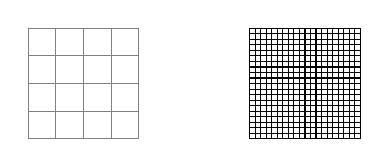
\begin{tikzpicture}[x=40pt,y=40pt]
            \draw[step=10pt,gray] (0,0) grid +(1,1);
            \draw[step=2pt]      (2,0) grid +(1,1);
        \end{tikzpicture}

        \medskip
        Even though the left grid comes first in English reading order, the
        right one is much more likely to be seen first: The white-to-black
        contrast is higher than the gray-to-white contrast. In addition,
        there are more ``places'' adding to the overall contrast in the right
        grid.

        即使左边的网格在英文阅读顺序中排在前面,右边的网格更有可能首先被注意到:白到黑的对比度高于灰到白的对比度。此外,右边的网格中有更多的“位置”增加了总体对比度。

        Things like grids and, more generally, help lines usually should not
        grab the attention of the readers and, hence, should be typeset with
        a low contrast to the background. Also, a loosely-spaced grid is less
        distracting than a very closely-spaced grid.

        像网格和辅助线这样的元素通常不应该吸引读者的注意力,因此应该以低对比度与背景进行排版。此外,网格的间距较大比间距非常紧密的网格更不容易分散注意力。

    \item Dashed lines create many points at which there is black-to-white
        contrast. Dashed or dotted lines can be very distracting and, hence,
        should be avoided in general.

        虚线会在许多点上产生黑到白的对比度。虚线或点线可能非常分散注意力,因此通常应该避免使用。

Do not use different dashing patterns to differentiate curves in
        plots. You lose data points this way and the eye is not particularly
        good at ``grouping things according to a dashing pattern''. The eye
        is \emph{much} better at grouping things according to colors.

        不要使用不同的虚线样式来区分图表中的曲线。这样你会丢失数据点,并且眼睛并不特别擅长“根据虚线样式分组事物”。眼睛在根据颜色分组事物方面要好得多。


    \item Background patterns filling an area using  diagonal lines or
        horizontal and vertical lines or just dots are almost always
        distracting and, usually, serve no real purpose.

        使用倾斜线、水平和垂直线或者点填充的背景图案几乎总是分散注意力的,通常没有实际用途。


    \item Background images and shadings distract and only seldomly add
        anything of importance to a graphic.

        背景图像和渐变会分散注意力,并且很少对图形添加重要信息。


    \item Cute little clip arts can easily draw attention away from the data.

    可爱的小图标很容易将注意力从数据上吸引走。


\end{itemize}
